\chapter{Multiple Integrals}


In this chapter, we extend this powerful idea into higher dimensions using the 
tools of multiple integration. While single integration enables us to calculate
the area under a curve or the volume under a surface, multiple integration 
allows us to calculate volumes in three dimensions, and even hypervolumes in 
higher dimensions.

We start by discussing double integration, which allows us to find the volume 
under a surface in three dimensions. This method involves slicing the solid 
into infinitesimally small columns, and summing the volumes of these columns.

Next, we'll cover triple integration, a tool that lets us find the volume of 
more complicated solids in three-dimensional space. The idea is similar to 
double integration.

To properly implement these techniques, we'll also discuss the different 
coordinate systems that can be used in multiple integration, such as 
rectangular, cylindrical, and spherical coordinates, and when it's advantageous
to use one system over another.

By the end of this chapter, you will have a deeper understanding of the 
techniques of multiple integration and how to apply them to find the volumes 
of various types of solids. The methods we study here will serve as a 
foundation for many topics in higher mathematics and physics, including 
electromagnetism, fluid dynamics, and quantum mechanics.

\section{Double Integrals}
[fixme intro paragraph]

\subsection{Over Rectangular Regions}
Suppose there is some function, $z = f(x,y)$, that is defined over the 
rectangular region, \textit{R}, defined by $\textit{R} = [a, b] \times [c,d] = 
\{(x,y)| a \leq x \leq b, c \leq y \leq d\}$, and $f$ is such that $f \geq 0$ 
for all $(x, y) \in \mathbb{R}$. Then the graph of $f$ is a surface that lies 
above the rectangular region, \textit{R} (see figure \ref{fig:f_on_R}). 

\begin{figure}[htbp]
    \centering
    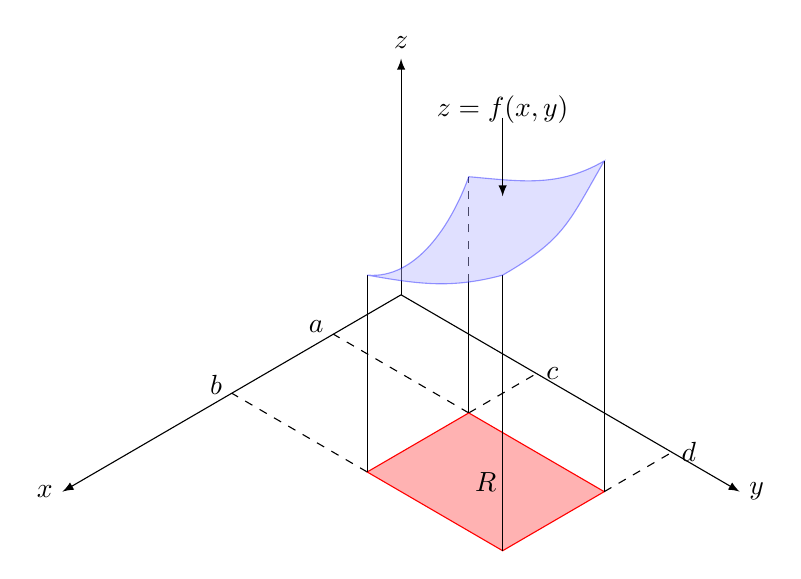
\begin{tikzpicture}[x = {(-0.86cm, -0.5cm)}, y = {(0.86cm, -0.5cm)}, 
    z = {(0cm, 1cm)}]
        \draw[-latex] (0,0,0) -- (5,0,0) node[left] {$x$};
        \draw[-latex] (0,0,0) -- (0,5,0) node[right] {$y$};
        \draw[-latex] (0,0,0) -- (0,0,3) node[above] {$z$};
        \draw[dashed] (1, 2, 0) -- (1, 0, 0) node[left, yshift = 0.1cm] {$a$};
        \draw[dashed] (2.5, 2, 0) -- (2.5, 0, 0) node[left, yshift = 0.1cm] 
        {$b$};
        \draw[dashed] (1, 2, 0) -- (0, 2, 0) node[right] {$c$};
        \draw[dashed] (1, 4, 0) -- (0, 4, 0) node[right] {$d$};
        \filldraw[draw = red, fill = red!30] (1, 2, 0) -- (2.5, 2, 0) -- 
        (2.5, 4, 0) -- (1, 4, 0) -- cycle;
        \node[] at (1.75, 3, 0) {$R$};
        \draw[] (2.5, 2, 0) -- (2.5, 2, 2.5);
        \draw[] (1, 2, 0) -- (1, 2, 1.66);
        \draw[dashed] (1, 2, 1.66) -- (1, 2, 3);
        \draw[] (2.5, 4, 0) -- (2.5, 4, 3.5);
        \draw[] (1, 4, 0) -- (1, 4, 4.2);
        \filldraw[draw = blue, fill = blue!30, opacity = 0.4] (2.5, 2, 2.5) 
        to[out = -5, in = -110, looseness = 0.9] (1, 2, 3) 
        to[out = -5, in = 210] (1, 4, 4.2) 
        to[out = 240, in = 30, looseness = 1.2] (2.5, 4, 3.5) 
        to[out = 195, in = -10] (2.5, 2, 2.5);
        \draw[-latex] (1, 2.5, 4) -- (1, 2.5, 3);
        \node[] at (1, 2.5, 4.1) {$z = f(x,y)$};
    \end{tikzpicture}
    \caption{The graph of $f$ over the region $R$}
    \label{fig:f_on_R}
\end{figure}

Let us call the solid that fills the space between the $xy$-plane and the 
surface $z = f(x,y)$ \textit{S}. Formally, this is written as
$$\textit{S} = \{ (x, y, z) \in \mathbb{R}^3 | 0 \leq z \leq f(x, y), (x, y) 
\in \mathbb{R}\}$$

How can we find the volume of the solid, \textit{S}? We will apply what we 
learned about Riemann sums and definite integrals in two dimensions to this 
three dimensional problem. 

First, we divide \textit{R} into rectangular subregions. We do this by 
dividing the interval $[a, b]$ into \textit{m} subintervals with width $\Delta 
x = (b - a)/m$ and the interval $[c, d]$ into \textit{n} subintervals with 
width $\Delta y = (d - c) / n$. Drawing lines through these divisions parallel 
to the $x$- and $y$-axes, we create a field of subrectangles, each with area 
$\Delta A = \Delta x \Delta y$ (see figure \ref{fig:subrectangles}). Each 
subrectangle is defined by:
$$\textit{R}_{ij} = [x_{i - 1}, x_i] \times [y_{j - 1}, y_j] - \{ (x, y) | x_{
i - 1} \leq x \leq x_i, y_{j - 1} \leq y \leq y_j \}$$ 

\begin{figure}[htbp]
    \centering
    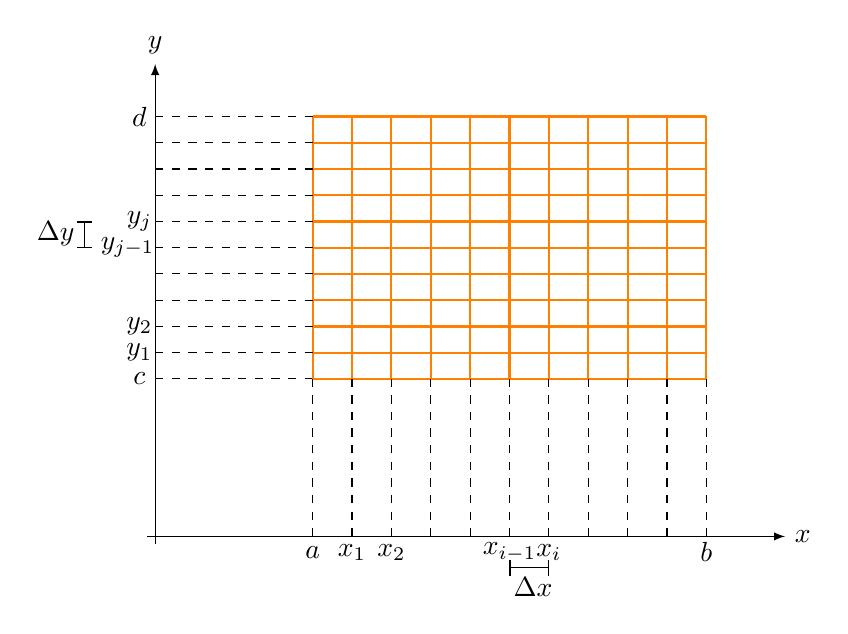
\begin{tikzpicture}
        \draw[-latex] (-0.1, 0) -- (8, 0) node[right] {$x$};
        \draw[-latex] (0, -0.1) -- (0, 6) node[above] {$y$};
        \foreach \i in {0,1, 2, 3, 4, 5, 6, 7, 8, 9, 10} {
            \draw[dashed] (2 + \i/2, 0) -- (2 + \i/2, 2);
            \draw[dashed] (0, 2 + \i/3) -- (2, 2 + \i/3);
            \draw[orange, thick] (2 + \i/2, 2) -- (2 + \i/2, 5.333);
            \draw[orange, thick] (2, 2 + \i/3) -- (7, 2 + \i/3);
            }
        \node[] at (2, -0.2) {$a$};
        \node[] at (7, -0.2) {$b$};
        \node[] at (2.5, -0.2) {$x_1$};
        \node[] at (3, -0.2) {$x_2$};
        \node[] at (4.5, -0.2) {$x_{i - 1}$};
        \node[] at (5, -0.2) {$x_i$};
        \draw[|-|] (4.5, -0.4) -- (5, -0.4) node[below, xshift = -0.2cm] 
        {$\Delta x$};
        \node[] at (-0.2, 2) {$c$};
        \node[] at (-0.2, 5.333) {$d$};
        \node[] at (-0.2, 2.333) {$y_1$};
        \node[] at (-0.2, 2.667) {$y_2$};
        \node[] at (-0.35, 3.667) {$y_{j - 1}$};
        \node[] at (-0.2, 4) {$y_j$};
        \draw[|-|] (-0.9, 3.667) -- (-0.9, 4) node[left, yshift = -0.15cm] 
        {$\Delta y$};
    \end{tikzpicture}
    \caption{The region, \textit{R}, on the $xy$-plane divided into 
    subrectangles}
    \label{fig:subrectangles}
\end{figure}

Since $f(x,y)$ in continuous over the \textit{R}, there is some point, $(x_{ij}
^*, y_{ij}^*)$, equal to the average value of $f(x,y)$ over the subrectangle. 
Then we can approximate the volume between the $xy$-plane and $z = f(x,y)$ over
the subrectangle as a column with base area $\Delta A$ and height $f(x_{ij}^*, 
y_{ij}^*)$ (seefigure \ref{fig:one_column}) and the volume of the column is 
given by:
$$V_{ij} = f(x_{ij}^*, y_{ij}^*) \Delta A$$

\begin{figure}[htbp]
    \centering
    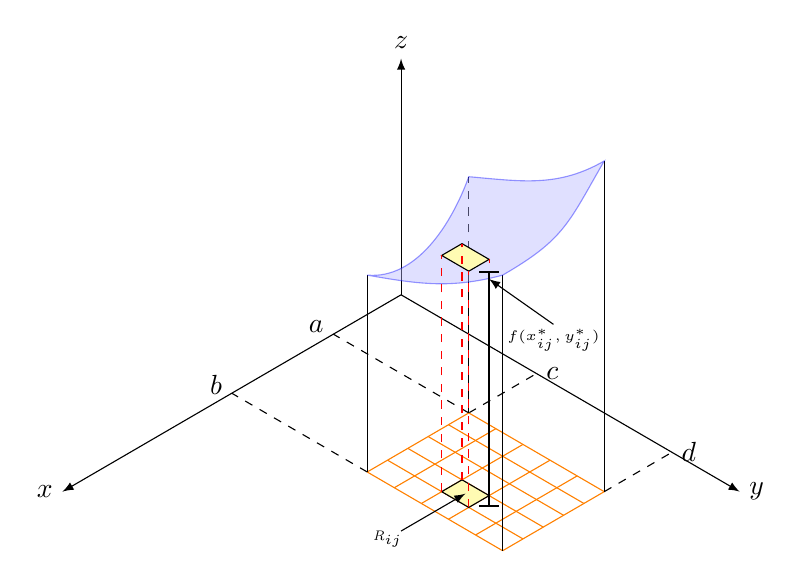
\begin{tikzpicture}[x = {(-0.86cm, -0.5cm)}, y = {(0.86cm, -0.5cm)}, 
    z = {(0cm, 1cm)}]
        \draw[-latex] (0,0,0) -- (5,0,0) node[left] {$x$};
        \draw[-latex] (0,0,0) -- (0,5,0) node[right] {$y$};
        \draw[-latex] (0,0,0) -- (0,0,3) node[above] {$z$};
        \draw[dashed] (1, 2, 0) -- (1, 0, 0) node[left, yshift = 0.1cm] {$a$};
        \draw[dashed] (2.5, 2, 0) -- (2.5, 0, 0) node[left, yshift = 0.1cm] 
        {$b$};
        \draw[dashed] (1, 2, 0) -- (0, 2, 0) node[right] {$c$};
        \draw[dashed] (1, 4, 0) -- (0, 4, 0) node[right] {$d$};
        \foreach \i in {0, 1, 2, 3, 4, 5} {
            \draw[orange] (1 + \i*1.5/5, 2, 0) -- (1 + \i*1.5/5, 4, 0);
            \draw[orange] (1, 2 + 2*\i/5, 0) -- (2.5, 2 + 2*\i/5, 0);
        }
        \draw[] (2.5, 2, 0) -- (2.5, 2, 2.5);
        \draw[] (1, 2, 0) -- (1, 2, 1.66);
        \draw[dashed] (1, 2, 1.66) -- (1, 2, 3);
        \draw[] (2.5, 4, 0) -- (2.5, 4, 3.5);
        \draw[] (1, 4, 0) -- (1, 4, 4.2);
        \filldraw[draw = blue, fill = blue!30, opacity = 0.4] (2.5, 2, 2.5) 
        to[out = -5, in = -110, looseness = 0.9] (1, 2, 3) 
        to[out = -5, in = 210] (1, 4, 4.2) 
        to[out = 240, in = 30, looseness = 1.2] (2.5, 4, 3.5) 
        to[out = 195, in = -10] (2.5, 2, 2.5);
        \filldraw[draw = black, fill = yellow!30] (1.9, 2.8, 0) -- 
        (1.9, 3.2, 0) -- (2.2, 3.2, 0) -- (2.2, 2.8, 0) -- cycle;
        \filldraw[draw = black, fill = yellow!30] (1.9, 2.8, 3) -- 
        (1.9, 3.2, 3) -- (2.2, 3.2, 3) -- (2.2, 2.8, 3) -- cycle;
        \foreach \x/\y in {1.9/2.8, 1.9/3.2, 2.2/3.2, 2.2/2.8} {
            \draw[red, dashed] (\x, \y, 0) -- (\x, \y, 3);
        }
        \draw[|-|, thick] (2.05, 3.35, 0) -- (2.05, 3.35, 3);
        \node[font = \tiny] at (0.75, 3, 1.3) {$f(x_{ij}^*, y_{ij}^*)$};
        \draw[-latex] (0.75, 3, 1.5) -- (2.05, 3.35, 2.9);
        \draw[-latex] (3, 3, 0) -- ( 2.05, 3, 0);
        \node[font = \tiny] at (3.2, 3, 0) {$\textit{R}_{ij}$};
    \end{tikzpicture}
    \caption{A single column with base $\Delta A$ and height $f(x_{ij}^*, 
    y_{ij}^*)$}
    \label{fig:one_column}
\end{figure}

And therefore the approximate volume of the solid, \textit{S}, that lies 
between the region, \textit{R}, and $z = f(x,y)$ is the sum of all the columns 
over $i$ and $j$:
$$V_{\textit{S}} \approx \sum_{i = 1}^n \sum_{j = 1}^n f(x_{ij}^*, y_{ij}^*) 
\Delta A$$

And just like with the area under a curve, we get the true volume by taking the
limit as $n \to \infty$, which becomes a \textbf{double integral}\index{double 
integral}:

\begin{mdframed}[style = important, frametitle = {Volume of a Solid over a 
Region}]
$$V_{\textit{S}} = \lim_{n \to \infty} \sum_{i = 1}^n \sum_{j = 1}^n f(x_{ij}^*
, y_{ij}^*) \Delta A = \iint_{\textit{R}} f(x, y)\,dA$$
\end{mdframed}

Note: a double integral is an integral performed in 2 dimensions at once. It is
not the same as two integrals nested within each other, which we will discuss 
below. 

\section{Iterated Integrals}

To be able to evaluate the double integral as outlined above, we must first 
discuss iterated integrals. Iterated integrals happen when you evaluate two 
single integrals, one inside the other. Consider some function, $g(x, y)$. We 
could integrate that function from $x = q$ to $x = r$ thusly:
$$\int_q^r g(x, y)\,dx$$
Notice that we are integrating with respect to $x$, so $y$ terms will be 
treated as constants (recall partial differentiation: this is the opposite 
process). Let's call the result of this first integral $A(y)$:
$$A(y) = \int_q^r g(x, y)\,dx$$

We can then integrate the resulting function, $A(y)$, from $y = s$ to $y = t$:
$$\int_s^t A(y)\,dy = \int_s^t \left[ \int_q^r g(x, y)\,dx \right]\,dy$$
This is called an \textbf{iterated integral}\index{iterated integral}. When 
evaluating iterated integrals, we work from the inside out. You can also write 
it without the brackets:
$$\int_s^t \int_q^r g(x, y)\,dx\,dy$$

\textbf{Example}: evaluate the iterated integral $\int_0^3 \int_1^2 x y^2\,dy
\,dx$.

\textbf{Solution}: We can re-write this to more explicitly show the inner and 
outer integrals:
$$\int_0^3 \left[ \int_1^2 x y^2\,dy \right]\,dx$$
As you can see, the inner integral is with respect to $y$. Let's isolate and 
evaluate the inner integral:
$$\int_1^2 x y^2\,dy = x \int_1^2 y^2\,dy = x \left[ \frac{1}{3}y^2 \right]_{y 
= 1}^{y = 2}$$
$$= \frac{x}{3} \left[ 2^3 - 1^3 \right] = \frac{x}{3} \left[ 8 - 1 \right] = 
\frac{7x}{3}$$

We were able to move $x$ outside the integral because when we are integrating 
with respect to a specific variable (in this case, $y$), other variables are 
treated as constants. Now we can substitute $\int_1^2 xy^2 \,dy = \frac{7x}{3}$
into the iterated integral:
$$\int_0^3 \left[ \int_1^2 x y^2\,dy \right]\,dx = \int_0^3 \left[ \frac{7x}{3}
\right]\,dx$$
$$= \frac{7}{3} \left[ \frac{1}{2}x^2 \right]_{x = 0}^{x = 3} = \frac{7}{6} 
\left[ 3^2 - 0^2 \right] = \frac{7 \cdot 9}{6} = \frac{21}{2}$$

\begin{Exercise}[title = {Order of Evaluating Iterated Integrals}, label = 
iterate 1]
Show that $\int_0^3 \int_1^2 x y^2\,dy\,dx = \int_1^2 \int_0^3 x y^2 \,dx\,dy$.
\end{Exercise}

\begin{Answer}[ref = iterate_1]
We have already shown that $\int_0^3 \int_1^2 x y^2\,dy\,dx = \frac{21}{2}$. 
We will evaluate $\int_1^2 \int_0^3 x y^2 \,dx\,dy$ and see if we get the same 
result. 
$$\int_0^3 x y^2 \,dx = y^2 \int_0^3 x\,dx = y^2 \left[ \frac{1}{2}x^2 \right]_
{x = 0}^{x = 3}$$
$$= \frac{y^2}{2} \left[ 3^2 - 0^2 \right] = \frac{9y^2}{2}$$
Substituting this back into the iterated integral:
$$\int_1^2 \int_0^3 x y^2 \,dx\,dy = \int_1^2 \frac{9y^2}{2}\,dy = \frac{9}{2} 
\int_1^2 y^2 \,dy$$
$$= \frac{9}{2} \left[ \frac{1}{3}y^3 \right]_{y = 1}^{y = 2} = \frac{9}{2} 
\cdot \frac{1}{3} \left[ 2^3 - 1^3 \right]$$
$$= \frac{3}{2}(8 - 1) = \frac{21}{2}$$
\end{Answer}

\begin{Exercise}[title = {Evaluating Iterated Integrals}, label = iterate_2]
Evaluate the following iterated integrals.
\begin{enumerate}
\item $\int_0^1 \int_1^2 \left( x + e^{-y} \right)\,dx\,dy$
\item $\int_{-3}^3 \int_{0}^{\pi/2} \left( 2y + y^2 \cos{x} \right)\,dx\,dy$
\item $\int_0^3 \int_0^{\pi/2} t^2 \sin^3{\theta}\,d\theta\,dt$
\end{enumerate}
\vspace{100mm}
\end{Exercise}

\begin{Answer}[ref = iterate_2]
\begin{enumerate}
\item Answer: $\frac{5}{2} - \frac{1}{e}$. Solution: $\int_0^1 \int_1^2 \left( 
x + e^{-y} \right)\,dx\,dy = \int_0^1 \left( \frac{1}{2}x^2 + xe^{-y} \right)
|_{x=1}^{x=2}\,dy = \int_0^1 \left( 2 - \frac{1}{2} + 2e^{-y} - e^{-y} \right)
\,dy = \int_0^1 \left( \frac{3}{2} + e^{-y} \right)\,dy = \left[ \frac{3}{2}y 
- e^{-y} \right]_{y = 0}^{y = 1} = \left( \frac{3}{2}(1) - e^{-1} \right) - 
\left( \frac{3}{2}(0) - e^0 \right) = \frac{5}{2} - \frac{1}{e}$
\item Answer: $18$. Solution: $\int_{-3}^3 \int_{0}^{\pi/2} \left( 2y + y^2 
\cos{x} \right)\,dx\,dy = \int_{-3}^3 \left[ 2xy + y^2 \sin{x} \right]_{x = 0}^
{x = \pi/2}\,dy = \int_{-3}^3 \left[ \left( \pi y + y^2 \right) - \left( 0 + 0 
\right) \right]\,dy = \int_{-3}^3 \left( \pi y + y^2 \right)\,dy = \left[ 
\frac{\pi}{2}y^2 + \frac{1}{3}y^3 \right]_{y = -3}^{y = 3} = \left( \frac{\pi}{
2}(9) + \frac{1}{3}(27) \right) - \left( \frac{\pi}{2}(9) + \frac{1}{3}(-27) 
\right) = 9 - (-9) = 18$
\item Answer: $6$. Solution: $\int_0^3 \int_0^{\pi/2} t^2 \sin^3{\theta}\,
d\theta\,dt = \left( \int_0^3 t^2\,dt \right) \times \left( \int_0^{\pi/2} 
\sin^3{\theta}\,d\theta \right) = \left[ \frac{1}{3}t^3 \right]_{t = 0}^{t = 3}
\times \left( \int_0^{\pi/2} \sin{\theta} \sin^2{\theta}\,d\theta \right) = 9
\int_0^{\pi/2} \sin{\theta} \left( 1 - \cos^2{\theta} \right)\,d\theta = 9 
\left[ \int_0^{\pi/2} \sin{\theta}\,d\theta - \int_0^{\pi/2} \sin{\theta}
\cos^2{\theta}\,d\theta \right] = 9 \left[ \left( -\cos{\theta} \right) |_{
\theta = 0}^{\theta = \pi/2} + \left( \frac{1}{3}\cos^3{\theta} \right)|_{
\theta = 0}^{\theta = \pi/2} \right] = 9 \left[ -(-\cos{0}) + (-\frac{1}{3}
\cos^3{0}) \right] = 9 \left( 1 - \frac{1}{3} \right) = 9 \left( \frac{2}{3} 
\right) = 6$
\end{enumerate}
\end{Answer}

\section{Fubini's Theorem for Double Integrals}

As stated above, a double integral is not quite the same thing as two iterated 
integrals. However, they are related. Fubini's theorem states that for a 
function, $f$, that is continuous over the rectangular region, \textit{R}, the 
double integral of $f$ over the region $\textit{R} = \{ (x, y) | a \leq x \leq 
b, c \leq y \leq d\}$ is equal to the iterated integral of $f$ with respect to 
$x$ and $y$. This is expressed mathematically below:

\begin{mdframed}[style = important, frametitle = {Fubini's Theorem}]
If $f$ is continuous on the rectangle $R = \{ \left( x, y \right) | a \leq x 
\leq b, c \leq y \leq d \}$, then
$$\iint_R f(x,y)\,\,dA = \int_a^b \int_c^d f(x,y)\,dy\,dx = \int_c^d \int_a^b 
f(x,y)\,dx\,dy$$
\end{mdframed}

\begin{Exercise}[title={Applying Fubini's Theorem},label = fubini_1]
Rewrite the following double integrals as iterated integrals.
\begin{enumerate}
\item $\iint_R \frac{xy^2}{x^2 + 1}\,\,dA$, $R = \{(x,y)|0 \leq x \leq 1, -3 
\leq y \leq 3\}$
\item $\iint_R \frac{\sec{\theta}}{\sqrt{1 + t^2}}\,\,dA$, $R = \{(\theta, t) |
0 \leq \theta \leq \frac{\pi}{4}, 0 \leq t \leq 1 \}$
\end{enumerate}
\vspace{40mm}
\end{Exercise}

\begin{Answer}[ref = fubini_1]
\begin{enumerate}
\item $\int_0^1 \int_{-3}^3 \frac{xy^2}{x^2 + 1}\,dy\,dx$ OR $\int_{-3}^3 
\int_0^1 \frac{xy^2}{x^2 + 1}\,dx\,dy$
\item $\int_0^{\pi/4} \int_0^1 \frac{\sec{\theta}}{\sqrt{1 + t^2}}\,dt\,
d\theta$ OR $\int_0^1 \int_0^{\pi/4} \frac{\sec{\theta}}{\sqrt{1 + t^2}}\,
d\theta \,dt$
\end{enumerate}
\end{Answer}

\begin{Exercise}[label = fubini_2]
Evaluate the double integral. 
\begin{enumerate}
\item $\iint_R \frac{xy^2}{x^2 + 1}\,dA$, $\textit{R} = \{ \left( x, y \right) 
| \text{ } 0 \leq x \leq 2, \text{ } -3 \leq y \leq 3 \}$
\item $\iint_R \frac{\tan{\theta}}{\sqrt{1 - t^2}}\,dA$, $\textit{R} = \{ 
\left( \theta, t \right) | \text{ } 0 \leq \theta \leq \pi/3, \text{ } 0 \leq 
t \leq \frac{1}{2} \}$
\item $\iint_R x \sin{ \left( x + y \right) }\,dA$, $\textit{R} = \left[0, 
\pi/6 \right] \times \left[ 0, \pi/3 \right]$
\end{enumerate}
\end{Exercise}

\begin{Answer}[ref = fubini_2]
\begin{enumerate}
\item $\iint_R \frac{xy^2}{x^2 + 1}\,dA$, $\textit{R} = \{ \left( x, y \right) 
| 0 \leq x \leq 2, -3 \leq y \leq 3 \} = \int_0^2 \int_{-3}^3 \frac{xy^2}{x^2 
+ 1}\,dy\,dx = \int_0^2 \frac{x}{x^2 + 1}\,dx \cdot \int_{-3}^{3} y^2\,dy$. To 
evaluate the integral with respect to $x$, we use the $u$-substitution $u = 
x^2 + 1$, $(x)dx = \frac{1}{2} du$: $\int_0^2 \frac{x}{x^2 + 1}\,dx \cdot 
\int_{-3}^{3} y^2\,dy = \int_{x = 0}^{x = 2} \frac{1}{2} \frac{1}{u}\,du \cdot 
\int_{-3}^3 y^2\,dy = \frac{1}{2} \ln{|u|}|_{x = 0}^{x = 2} \cdot \frac{1}{3} 
\left[ y^3 \right]_{y = -3}^{y = 3} = \frac{1}{2} \left[ \ln{\left( 2^2 + 1 
\right) - \ln{ \left( 0^2 + 1 \right)}} \right] \cdot \frac{1}{3} \left[ 3^3 - 
\left( -3 \right)^3 \right] = \frac{1}{2} \ln{5} \cdot \frac{1}{3} \left( 27 - 
(-27) \right) = \frac{\ln{5}}{2} \frac{54}{3} = 9\ln{5}$
\item $\iint_R \frac{\tan{\theta}}{\sqrt{1 - t^2}}\,dA$, $\textit{R} = \{ 
\left( \theta, t \right) | \text{ } 0 \leq \theta \leq \pi/3, \text{ } 0 \leq 
t \leq \frac{1}{2} \} = \int_0^{\pi/3} \int_0^{1/2} \frac{\tan{\theta}}{\sqrt{
1 - t^2}}\,dt\,d\theta = \left[ \int_0^{\pi/3} \tan{\theta}\,d\theta \right] 
\cdot \left[ \int_0^{1/2} \frac{1}{\sqrt{1 - t^2}}\,dt \right]$. Recall that 
$\frac{d}{dt} \arcsin{t} = \frac{1}{\sqrt{1 - t^2}}$. Applying FTC, then 
$\left[ \int_0^{\pi/3} \tan{\theta}\,d\theta \right] \cdot \left[ \int_0^{1/2} 
\frac{1}{\sqrt{1 - t^2}}\,dt \right] = \left[ \int_0^{\pi/3} \tan{\theta}\,d\theta 
\right] \cdot \left[ \arcsin{t} \right]_{t = 0}^{t = 1/2} = \left[ \int_0^{\pi/
3} \tan{\theta}\,d\theta \right] \cdot \left[ \arcsin{\frac{1}{2}} - \arcsin{0}
\right] = \left[ \int_0^{\pi/3} \tan{\theta}\,d\theta \right] \cdot \left[ 
\frac{\pi}{6} \right] = \frac{\pi}{6} \int_0^{\pi/3} \frac{\sin{\theta}}{\cos{
\theta}}\,d\theta$. To evaluate this final integral, we use the $u$-substitution
$u = \cos{\theta}$ and $-du = \sin{\theta} d\theta$: $\frac{\pi}{6} \int_0^{\pi
/3} \frac{\sin{\theta}}{\cos{\theta}}\,d\theta = -\frac{\pi}{6}\int_{\theta = 0
}^{\theta = \pi/3} \frac{1}{u}\,du = -\frac{\pi}{6} \ln{u}|_{\theta = 0}^{
\theta = \pi/3} = -\frac{\pi}{6} \left[ \ln{ \left( \cos{\theta} \right)} 
\right]_{\theta = o}^{\theta = \pi/3} = \frac{\pi}{6} \left[ \ln{\left( \cos{0} 
\right) - \ln{ \left( \cos{\frac{\pi}{3}} \right)}} \right] = \frac{\pi}{6} 
\left[ \ln{1} - \ln{\frac{1}{2}} \right] = \frac{\pi}{6} \ln{\frac{1}{1/2}} = 
\frac{\pi}{6} \ln{2}$
\item $\iint_R x \sin{ \left( x + y \right) }\,dA$, $\textit{R} = \left[0, 
\pi/6 \right] \times \left[ 0, \pi/3 \right] = \int_0^{\pi/6} \int_0^{\pi/3} x 
\sin{ \left( x + y \right) }\,dy\,dx$. Recall the sum formula for sine:
$$\sin{ \left( x + y \right)} = \sin{x}\cos{y} + \cos{x}\sin{y}$$

We can substitute this into our iterated integral:
$$\int_0^{\pi/6} \int_0^{\pi/3} x \sin{ \left( x + y \right) }\,dy\,dx = 
\int_0^{\pi/6} \int_0^{\pi/3} x \left[ \sin{x}\cos{y} + \cos{x}\sin{y} 
\right]\,dy\,dx$$
$$= \int_0^{\pi/6} \left[ \int_0^{\pi/3} x \sin{x} \cos{y}\,dy + \int_0^{\pi/3}
x \cos{x} \sin{y}\,dy \right]\,dx$$

Let us designate $\int_0^{\pi/3} x \sin{x} \cos{y}\,dy$ as integral \textbf{A} 
and $\int_0^{\pi/3} x \cos{x} \sin{y}\,dy$ as integral \textbf{B}. First, we 
will evaluate integral \textbf{A}:
$$\int_0^{\pi/3} x \sin{x} \cos{y}\,dy = x \sin{x} \int_0^{\pi/3} \cos{y}\,dy$$
$$= x \sin{x} \left[ \sin{y} \right]_{y = 0}^{y = \pi/3} = x \sin{x} \left[ 
\sin{\frac{\pi}{3}} - \sin{0} \right]$$
$$= x \sin{x} \left( \frac{\sqrt{3}}{2} \right) = \frac{x \sqrt{3}}{2} \sin{x}$$

Next we evaluate integral \textbf{B}:
$$\int_0^{\pi/3} x \cos{x} \sin{y}\,dy = x \cos{x} \int_0^{\pi/3} \sin{y}\,dy$$
$$= x \cos{x} \left[ - \cos{y} \right]_{y = 0}^{y = \pi/3} = x \cos{x} \left[ -
\cos{\frac{\pi}{3}} - \left( - \cos{0} \right) \right]$$
$$= x\cos{x} \left[ - \frac{1}{2} - (-1) \right] = \frac{x}{2}\cos{x}$$

Substituting back in for integrals \textbf{A} and \textbf{B}:
$$\int_0^{\pi/6} \left[ \int_0^{\pi/3} x \sin{x} \cos{y}\,dy + \int_0^{\pi/3} 
x \cos{x} \sin{y}\,dy \right]\,dx = \int_0^{\pi/6} \left[ \frac{x \sqrt{3}}{2} 
\sin{x} + \frac{x}{2}\cos{x} \right]\,dx$$
$$= \frac{\sqrt{3}}{2} \int_0^{\pi/6} x \sin{x}\,dx + \frac{1}{2} \int_0^{
\pi/6} x \cos{x}\,dx$$

Again, we will designate $\int_0^{\pi/6} x \sin{x}\,dx$ as integral \textbf{C} 
and $\int_0^{\pi/6} x \cos{x}\,dx$ as integral \textbf{D}. We start by using 
integration by parts to evaluate integral \textbf{C}:

Let $u = x$ and $dv = \sin{x} dx$. Then $v = -cos{x}$ and $du = dx$ and 
therefore:
$$\int_0^{\pi/6} x \sin{x}\,dx = \left[ x \left(- \cos{x} \right) \right]_{x = 
0}^{x = \pi/6} - \int_0^{\pi/6} \left( - \cos{x} \right)\,dx$$
$$= \left[ \frac{\pi}{6} \left(- \cos{\frac{\pi}{6}} \right) \right] - \left[ 
0 \left(- \cos{0} \right) \right] + \sin{x}|_{x = 0}^{x = \pi/6}$$
$$= -\frac{\pi}{6} \cdot \frac{\sqrt{3}}{2} - 0 + \sin{\frac{\pi}{6}} - 
\sin{0} = \frac{1}{2} - \frac{\pi \sqrt{3}}{12} = \frac{6 - \pi \sqrt{3}}{12}$$

Next, we will use integration by parts to evaluate integral \textbf{D}. Let $u 
= x$ and $dv = \cos{x} dx$. Then $du = dx$ and $v = \sin{x}$ and therefore:
$$\int_0^{\pi/6} x \cos{x}\,dx = \left[ x \sin{x} \right]_{x = 0}^{x = \pi/6} -
\int_0^{\pi/6} \sin{x}\,dx$$
$$= \left[ \frac{\pi}{6}\sin{\frac{\pi}{6}} - 0\sin{0} \right] - \left( - 
\cos{x} \right)|_{x = 0}^{x = \pi/6} = \frac{\pi}{6} \cdot \frac{1}{2} + 
\cos{\frac{\pi}{6}} - \cos{0}$$
$$= \frac{\pi}{12} + \frac{\sqrt{3}}{2} - 1 = \frac{\pi + 6\sqrt{3} - 12}{12}$$

Substituting back in for integrals \textbf{C} and \textbf{D}:
$$\frac{\sqrt{3}}{2} \int_0^{\pi/6} x \sin{x}\,dx + \frac{1}{2} \int_0^{\pi/6} 
x \cos{x}\,dx = \frac{\sqrt{3}}{2} \left( \frac{6 - \pi \sqrt{3}}{12} \right) 
+ \frac{1}{2} \left( \frac{\pi + 6\sqrt{3}- 12}{12} \right)$$
$$= \frac{6 \sqrt{3} - 3\pi + \pi + 6\sqrt{3} - 12}{24} = \frac{6 \sqrt{3} - 6 
- \pi}{12}$$
\end{enumerate}
\end{Answer}

\section{Double Integrals over Non-Rectangular Regions}

Now that we've seen how to evaluate double integrals over rectangular regions, 
let's consider non-rectangular regions. Suppose we are interested in the 
integral of a function, $f(x,y)$, over a region, \textit{D}, exists such that 
it can be bounded by inside a rectangular region, \textit{R} (see figure 
\ref{fig:enclose}). We can then define a new function:
$$F(x, y) = 
\begin{cases}
	f(x, y) & \text{if } (x, y) \text{ is in \textit{D}}\\
	0 & \text{if } (x, y) \text{ is in \textit{R} but not in \textit{D}}
\end{cases}$$

\begin{figure}[htbp]
    \centering
    \begin{minipage}{0.45\textwidth}
        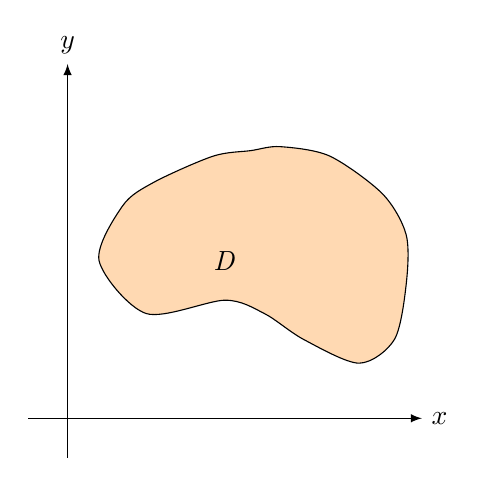
\begin{tikzpicture}
            \draw[-latex] (-0.5, 0) -- (4.5, 0) node[right] {$x$};
            \draw[-latex] (0, -0.5) -- (0, 4.5) node[above] {$y$};
            \draw[fill = orange!30] plot [smooth cycle] 
        coordinates {(0.4, 2) (0.7, 2.7) (1.1, 3) (1.85, 3.33) (2.33, 3.4) 
        (2.7, 3.45) (3.33, 3.33) (4, 2.85) (4.3, 2.33) (4.3, 1.7) (4.15, 1) 
        (3.7, 0.7) (3, 1) (2.5, 1.33) (2, 1.5) (1, 1.33)};
        \node[] at (2, 2) {\textit{D}};
        \end{tikzpicture}
    \end{minipage}
    \begin{minipage}{0.45\textwidth}
        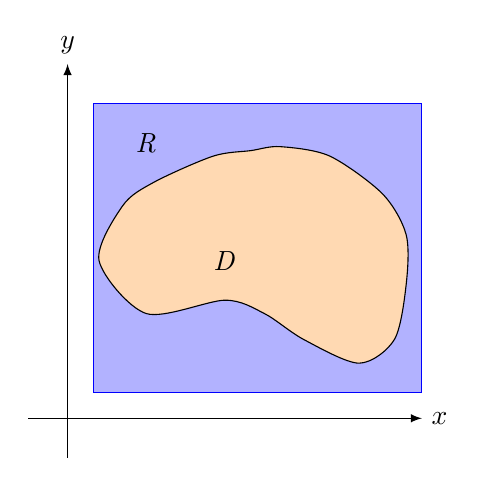
\begin{tikzpicture}
            \draw[-latex] (-0.5, 0) -- (4.5, 0) node[right] {$x$};
            \draw[-latex] (0, -0.5) -- (0, 4.5) node[above] {$y$};
            \draw[blue, fill = blue!30] (0.33, 0.33) rectangle (4.5, 4);
            \draw[fill = orange!30] plot [smooth cycle] 
        coordinates {(0.4, 2) (0.7, 2.7) (1.1, 3) (1.85, 3.33) (2.33, 3.4) 
        (2.7, 3.45) (3.33, 3.33) (4, 2.85) (4.3, 2.33) (4.3, 1.7) (4.15, 1) 
        (3.7, 0.7) (3, 1) (2.5, 1.33) (2, 1.5) (1, 1.33)};
        \node[] at (2, 2) {\textit{D}};
        \node[] at (1, 3.5) {\textit{R}};
        \end{tikzpicture}
    \end{minipage}
    \caption{We can find a rectangular region, \textit{R}, that completely 
    encloses \textit{D}}
    \label{fig:enclose}
\end{figure}

Then, we can see that:
$$\iint_{\textit{D}} f(x, y)\,dA = \iint_{\textit{R}} F(x, y)\,dA$$

Which makes sense intuitively, since integrating over $F$ outside of \textit{D}
doesn't contribute anything to the integral, and the integral of $F$ inside 
\textit{D} is equal to the integral of $f$ inside \textit{D}. In general, there
are two types of regions for \textit{D}. A region is \textbf{type I} if it lies
between two continuous functions of $x$ and can be defined thusly:
$$\textit{D} = \{ (x, y) \text{ } | \text{ } a \leq x \leq b, g_1(x) \leq y 
\leq g_2(x) \}$$

\begin{figure}[htbp]
    \centering
    \begin{minipage}{0.5\textwidth}
        \begin{tikzpicture}
            \begin{axis}[ymin = -0.3, ymax = 4, xmin = -0.3, xmax = 3, 
            axis lines = center, ticks = none, xlabel = $x$, ylabel = $y$] 
                \addplot[name path = A, domain = 0.5:2.5, orange, thick] {
                (0.5*x - 0.75)^2 + 0.5};
                \addplot[name path = B, domain = 0.5:2.5, orange, thick] {
                (x-2)^3 + 2*(x-2)^2 + x -1 + 1.5};
                \addplot[fill = orange!30] fill between [of = A and B];
                \draw[orange, thick] (0.5, 0.75) -- (0.5, 2.12);
                \draw[orange, thick] (2.5, 0.75) -- (2.5, 3.65);
                \draw[dashed] (0.5, 0.75) -- (0.5, 0) node[below] {$a$};
                \draw[dashed] (2.5, 0.75) -- (2.5, 0) node[below] {$b$};
                \node[] at (1.5, 2.8) {$y = g_2 (x)$};
                \node[] at (1.75, 0.25) {$y = g_1 (x)$};
                \node[] at (1.5, 1.5) {\textit{D}};
            \end{axis}
        \end{tikzpicture}
    \end{minipage}
    
    \begin{minipage}{0.5\textwidth}
        \begin{tikzpicture}
            \begin{axis}[ymin = -0.3, ymax = 4, xmin = -0.3, xmax = 3, 
            axis lines = center, ticks = none, xlabel = $x$, ylabel = $y$] 
                \addplot[name path = A, domain = 0.5:2.5, orange, thick, 
                samples = 150] {1.75 + sqrt(x - 0.5)};
                \addplot[name path = B, domain = 0.5:2.5, orange, thick, 
                samples = 150] {1.75 - sqrt(x - 0.5)};
                \addplot[fill = orange!30] fill between [of = A and B];
                \draw[orange, thick] (2.5, 0.33) -- (2.5, 3.17);
                \draw[dashed] (0.5, 1.75) -- (0.5, 0) node[below] {$a$};
                \draw[dashed] (2.5, 0.33) -- (2.5, 0) node[below] {$b$};
                \node[] at (1.25, 3.1) {$y = g_2 (x)$};
                \node[] at (1.5, 0.25) {$y = g_1 (x)$};
                \node[] at (1.5, 1.5) {\textit{D}};
            \end{axis}
        \end{tikzpicture}
    \end{minipage}
    \caption{Two examples of type I domains}
    \label{fig:type1}
\end{figure}

Some type I regions are shown in figure \ref{fig:type1}. To evaluate $\iint_{
\textit{D}} f(x,y)\,dA$, we begin by choosing a rectangle $\textit{R} = \left[ 
a, b \right] \times \left[ c, d \right]$ such that \textit{D} is completely 
contained in \textit{R}. We again define $F(x, y)$ such that $F(x, y) = f(x,y)$
on \textit{D} and $F = 0$ outside of \textit{D}. Then, by Fubini's theorem:
$$\iint_{\textit{D}} f(x, y)\,dA = \iint_{\textit{R}} F(x, y)\,dA = \int_a^b 
\int_c^d F(x, y)\,dy\,dx$$

Since $F(x, y) = 0$ when $y \leq g_1(x)$ or $y \geq g_2(x)$, we know that:
$$\int_c^d F(x, y)\,dy = \int_{g_1(x)}^{g_2(x)} F(x, y)\,dy = \int_{g_1(x)}^{
g_2(x)} f(x, y)\,dy$$

Substituting this into the iterated integral above, we see that for a type I 
region $\textit{D} = \{ (x, y) \text{ } | \text{ } a \leq x \leq b, g_1(x) 
\leq y \leq g_2(x) \}$, 
$$\iint_{\textit{D}} f(x, y)\,dA = \int_a^b \int_{g_1(x)}^{g_2(x)} f(x, y)
\,dy\,dx$$

A \textbf{type II} region is a region such that we can define the limits of 
$x$ in terms of $y$ (see figure \ref{fig:type2}). That is, a type II region 
can be defined as:
$$\textit{D} = \{(x, y) \text{ } | \text{ } c \leq y \leq d, h_1(y0 \leq x 
\leq h_2(y) \}$$

And in a similar manner to above, we can show that:
$$\iint_{\textit{D}} f(x, y)\,dA = \int_c^d \int_{h_1(y)}^{h_2(y)} f(x, y)
\,dx\,dy$$

\begin{figure}[htbp]
    \centering
    \begin{minipage}{0.5\textwidth}
        \begin{tikzpicture}
            \begin{axis}[ymin = -0.3, ymax = 4, xmin = -0.3, xmax = 3, 
            axis lines = center, ticks = none, xlabel = $x$, ylabel = $y$] 
                
                \draw[orange, fill = orange!30] (0.8, 0.2) -- (2.41, 0.2) -- 
                (2.25, 0.35) -- (2.04, 0.5) -- (1.81, 0.65) -- (1.63, 0.8) -- 
                (1.52, 0.95) -- (1.505, 1) -- (1.5, 1.05) -- (1.506, 1.1) -- 
                (1.524, 1.15) -- (1.552, 1.2) -- (1.59, 1.25) -- (1.75, 1.4) -- 
                (1.97, 1.55) -- (2.19, 1.7) -- (2.37, 1.85) -- (2.417, 1.9) -- 
                (2.454, 1.95) -- (2.48, 2) -- (2.496, 2.05) -- (2.5, 2.1) -- 
                (2.493, 2.15) -- (2.475, 2.2) -- (2.447, 2.25) -- (2.41, 2.3) 
                -- (2.24, 2.45) -- (2.03, 2.6) -- (1.81, 2.75) -- (1.63, 2.9) 
                -- (0.365, 2.9) -- (0.247, 2.75) -- (0.158, 2.6) -- 
                (0.109, 2.45) -- (0.102, 2.4) -- (0.1, 2.35) -- (0.103, 2.3) 
                -- (0.111, 2.25) -- (0.124, 2.2) -- (0.142, 2.15) -- 
                (0.222, 2) -- (0.335, 1.85) -- (0.472, 1.7) -- (0.621, 1.55) 
                -- (0.767, 1.4) -- (0.899, 1.25) -- (1.004, 1.1) -- 
                (1.073, 0.95) -- (1.087, 0.9) -- (1.096, 0.85) -- (1.1, 0.8) 
                -- (1.099, 0.75) -- (1.093, 0.7) -- (1.083, 0.65) -- 
                (1.021, 0.5) -- (0.922, 0.35) -- (0.795, 0.2) -- cycle;
                \addplot[name path = A, domain = 0.2:2.9, orange, thick, 
                samples = 100] (0.5*sin(deg(2*x)) + 0.6, x) ;
                \addplot[name path = B, domain = 0.2:2.9, orange, thick, 
                samples = 100] (0.5*cos(deg(3*x)) + 2, x);
                \draw[orange, thick] (0.8, 0.2) -- (2.41, 0.2);
                \draw[orange, thick] (0.365, 2.9) -- (1.63, 2.9);
                \draw[dashed] (0.795, 0.2) -- (0, 0.2) node[left] {$a$};
                \draw[dashed] (0.365, 2.9) -- (0, 2.9) node[left] {$b$};
                \node[] at (2.5, 1.5) {$x = h_2 (x)$};
                \node[] at (0.6, 1.0) {$x = h_1 (x)$};
                \node[] at (1.3, 2) {\textit{D}};
            \end{axis}
        \end{tikzpicture}
    \end{minipage}
    
    \begin{minipage}{0.5\textwidth}
        \begin{tikzpicture}
            \begin{axis}[ymin = -0.3, ymax = 4, xmin = -0.3, xmax = 3, 
            axis lines = center, ticks = none, xlabel = $x$, ylabel = $y$] 
                \draw[orange, fill = orange!30] (0.865, 2.9) -- (2.475, 2.9) 
                -- (2.396, 2.6) -- (2.317, 2.3) -- (2.232, 2) -- (2.143, 1.7) 
                -- (2.049, 1.4) -- (1.949, 1.1) -- (1.842, 0.8) -- (1.725, 0.5) 
                -- (1.638, 0.295) -- (1.529, 0.5) -- (1.404, 0.8) -- 
                (1.301, 1.1) -- (1.211, 1.4) -- (1.131, 1.7) -- (1.057, 2) -- 
                (0.989, 2.3) -- (0.925, 2.6) -- cycle;
                \addplot[name path = A, domain = 0.295:2.9, orange, thick, 
                samples = 150] (sqrt(x + 1) + 0.5, x);
                \addplot[name path = B, domain = 0.295:2.9, orange, thick, 
                samples = 150] (-2*sqrt(x)/3 + 2, x);
                \draw[orange, thick] (0.865, 2.9) -- (2.475, 2.9);
                \draw[dashed] (1.638, 0.295) -- (0, 0.295) node[left] {$a$};
                \draw[dashed] (0.865, 2.9) -- (0, 2.9) node[left] {$b$};
                \node[] at (2.6, 1.7) {$x = h_2 (x)$};
                \node[] at (0.8, 1.25) {$x = h_1 (x)$};
                \node[] at (1.5, 1.5) {\textit{D}};
            \end{axis}
        \end{tikzpicture}
    \end{minipage}
    \caption{Two examples of type II domains}
    \label{fig:type2}
\end{figure}

\subsection{Determining Region Type}
Many regions can be described as type I or type II. Consider the region between the curves $y = \frac{3}{2}(x - 1)$ and $y = \frac{1}{2} (x - 1)^2$ (see figure \ref{fig:example1}).[fix me classifying domains examples and explanations]

\begin{figure}[htbp]
    \centering
        \begin{tikzpicture}
    \begin{axis}[xlabel = $x$, ylabel = $y$, axis lines = center, ticks = none,
    xmin = -0.2, xmax = 5, ymin = -0.2, ymax = 5, clip = false]
        \addplot[blue, thick, name path = A, domain = 1:4] {(3/2)*(x-1)};
        \addplot[blue, thick, samples = 100, name path = B, domain = 1:4] 
        {(x-1)^2/2};
        \addplot[blue!30, opacity = 0.4] fill between [of = A and B];
        \addplot[blue, thick, domain = 0.867:4.33] {(3/2)*(x-1)};
        \addplot[blue, thick, samples = 100, domain = -0.2:4.16] {(x-1)^2/2};
        \node[] at (4, 2.5) {$y = \frac{(x - 1)^2}{2}$};
        \node[] at (1.5, 2) {$y = \frac{3(x-1)}{2}$};
        \addplot[blue, mark = *, only marks] coordinates {(4, 4.5) (1, 0)};
        \node[] at (4.5, 4.5) {$(4, 4.5)$};
        \node[] at (1.25, -0.3) {$(1, 0)$};
    \end{axis}
\end{tikzpicture}
    \caption{The region that lies between $y = \frac{(x - 1)^2}{2}$ and $y = 
    \frac{3(x - 1)}{2}$ can be classified as type I or type II}
    \label{fig:example1}
\end{figure}



\textbf{Example}: Evaluate $\iint_{\textit{D}} (2x + y)\,dA$, where \textit{D} 
is the region bounded by the parabolas $y = 3x^2$ and $y = 2 + x^2$. Region 
\textit{D} is shown in figure \ref{fig:parabola}. 

\begin{figure}[htbp]
\centering
    \begin{tikzpicture}
        \begin{axis}[ymin = 0, ymax = 4, xmin = -1.2, xmax = 1.2, axis lines = 
        center]
            \addplot[blue, thick, name path = A, domain = -1:1]{2 + x^2};
            \addplot[blue, thick, name path = B, domain = -1:1]{3*x^2};
            \addplot[blue, thick, domain = -1.2:1.2]{2 + x^2};
            \addplot[blue, thick, domain = -1.2:1.2]{3*x^2};
            \addplot[mark = *, only marks, blue] coordinates {(-1, 3) (1, 3)};
            \addplot[fill = orange!30, opacity = 0.4] fill between [of = A and B];
        \end{axis}
    \end{tikzpicture}
    \caption{Region \textit{D} is bounded above by $y = 2 + x^2$ and below by 
    $y = 3x^2$}
    \label{fig:parabola}
\end{figure}

\textbf{Solution}:This is a type I region, since for a given $x$, $y \in \left[
3x^2, 2 + x^2 \right]$. We can define region \textit{D} as $\textit{D} = \{(x, 
y) \text{ }|\text{ } -1 \leq x \leq 1, 3x^2 \leq y \leq 2 + x^2 \}$. Therefore, 
$$\iint_{\textit{D}} (2x + y)\,dA = \int_{-1}^1 \int_{3x^2}^{2 + x^2} \left(2x 
+ y \right)\,dy\,dx$$
$$= \int_{-1}^1 \left[ \int_{3x^2}^{2 + x^2} 2x\,dy + \int_{3x^2}^{2 + x^2} y
\,dy \right]\,dx$$
$$= \int_{-1}^{1} \left[ 2xy|_{y = 3x^2}^{y = 2 + x^2} + \frac{1}{2}y^2|_{y = 
3x^2}^{y = 2+x^2} \right]\,dx$$
$$= \int_{-1}^1 \left[ 2x \left( 2 + x^2 - 3x^2 \right) + \frac{1}{2} \left( 
(2 + x^2)^2 - (3x^2)^2 \right) \right]\,dx$$

$$= \int_{-1}^1 \left[ 2 + 4x + 2x^2 - 4x^3 - 4x^4 \right]\,dx$$
$$= \left[ 2x + 2x^2 + \frac{2}{3}x^3 - x^4 - \frac{4}{5}x^5 \right]_{x = -1}^{
x = 1}$$
$$= \left( 2 + 2 + \frac{2}{3} - 1 - \frac{4}{5} \right) - \left( -2 + 2 - 
\frac{2}{3} - 1 + \frac{4}{5} \right)$$
$$= 4 + \frac{4}{3} - \frac{8}{5} = \frac{56}{15}$$

\begin{Exercise}[title = {Double Integrals over Non-Rectangular Regions}, 
label = non-rect]
Evaluate the double integral.
\begin{enumerate}
\item $\iint_{\textit{D}} e^{-y^2} \,dA$, \textit{D} $= \{(x, y) \text{ } | 
\text{ } 0 \leq y \leq 3, 0 \leq x \leq 2y \}$.
\item $\iint_{\textit{D}} x \sin{y}\,dA$, \textit{D} is bounded by $y = 0$, 
$y = x^2$, $x = 2$. 
\item $\iint_{\textit{D}} \left(2y - x \right)\,dA$, \textit{D} is bounded by 
the circle with center at the origin and radius 3. 
\end{enumerate}
\end{Exercise}

\begin{Answer}[ref = non-rect]
\begin{enumerate}
    \item $\iint_{\textit{D}} e^{-y^2} \,dA = \int_0^3 \int_{0}^{2y} e^{-y^2}\,
    dx\,dy$ $= \int_0^3 \left[ e^{-y^2} x|_{x = 0}^{x = 2y} \right]\,dy$ $= 
    \int_0^3 2y e^{-y^2}\,dy$ $= -e^{-y^2}|_{y = 0}^{y = 3} = 1 - e^{-9} 
    \approx 0.9999$

    \item $\iint_{\textit{D}} x \sin{y}\,dA = \int_0^{2} \int_0^{x^2} x \sin{y}
    \,dy\,dx$ $= \int_0^{2} x \int_0^{x^2} \sin{y}\,dy\,dx$ $= \int_0^{2} x 
    \left[ -\cos{y} \right]_{y = 0}^{y = x^2}$ $= \int_0^{2} x \left( \cos{0} -
    \cos{x^2} \right)\,dx$ $= \int_0^{2} \left( x - x\cos{x^2} \right)\,dx$ $= 
    \left[ \frac{1}{2}x^2 - \frac{1}{2}\sin{x^2} \right]_{x = 0}^{x = 2}$ $= 
    \frac{1}{2}(2)^2 - \frac{1}{2} \left( \sin{2^2} - \sin{0} \right)$ $= 2 - 
    \frac{1}{2} \left( \sin{4} - 0 \right) = 2 - \frac{\sin{4}}{2} \approx 
    2.378$

    \item We can describe the region as \textit{D} $= \{ (x, y) \text{ } | 
    \text{ } -3 \leq x \leq -3, -\sqrt{9 - x^2} \leq y \leq \sqrt{9 - x^2} \}$.
    Therefore, $\iint_{\textit{D}} \left(2y - x \right)\,dA = \int_{-3}^3 
    \int_{-\sqrt{9 - x^2}}^{\sqrt{9 - x^2}} \left( 2x - y \right)\,dy\,dx$ $= 
    \int_{-3}^3 \left[ 2xy - \frac{1}{2}y^2 \right]_{y = -\sqrt{9 - x^2}}^{y = 
    \sqrt{9 - x^2}}\,dx$ $= \int_{-3}^3 \left[ 2x \left( \sqrt{9 - x^2} + 
    \sqrt{9 - x^2} \right) - \frac{1}{2} \left( 9 - x^2 - \left(9 - x^2 \right) 
    \right) \right]\,dx$ $= \int_{-3}^3 4x\sqrt{9 - x^2}\,dx$. Let $u = 9 - 
    x^2$, then $du = -2x$ and $4x = -2du$. Substituting, $\int_{-3}^3 4x\sqrt{
    9 - x^2}\,dx$ $= \int_{x = -3}^{x = 3} -2\sqrt{u}\,du$ $= -2 \cdot 
    \frac{2}{3} u^{3/2}|_{x = -3}^{x = 3}$ $= -\frac{4}{3} \left[ \left( 9 - 
    x^2 \right) \right]_{x = -3}^{x = 3} = 0$
\end{enumerate}
\end{Answer}

\section{Double Integrals in Other Coordinate Systems}
\begin{Exercise}[title={Using Polar Coordinates in Multiple Integration}, 
label=polarmulti]

\Question Use double integration to find the volume of the solid that lies 
under the surface $z = 4 - x^2 - y^2$ and above the $xy$-plane.

\end{Exercise}
\begin{Answer}[ref=polarmulti]

We are finding the volume of the solid that lies under the surface $z = 4 - 
x^2 - y^2$ and above the $xy$-plane.

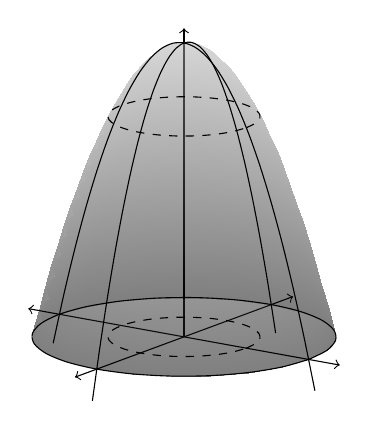
\begin{tikzpicture}
  \begin{axis}[
    view={35}{15},
    unit vector ratio=1 1 1,
    ticks = none,
    axis lines=middle,
    ymin=-2.5,
    ymax=2.5,
    xmax=2.5,
    xmin=-2.5,
    zmin=0,
    zmax=4.2,
    x axis line style=<->,
    y axis line style=<->,
    z axis line style=->,
    clip=false
  ]
    \addplot3[surf,shader=interp,domain=0:360,y domain=0:2, opacity=0.5,
    colormap={blackwhite}{color=(black) color=(black!30)}] ({y*cos(x)},
    {y*sin(x)},{4-y^2});
    \addplot3[samples y=0,domain=0:360,smooth]({2*cos(x)},  {2*sin(x)},0);
    \addplot3[samples y=0,domain=0:360,smooth,dashed]({cos(x)},  {sin(x)},0);
    \addplot3[samples y=0,domain=0:360,smooth,dashed]({cos(x)},  {sin(x)},3);
    \addplot3[samples y=0,domain=-2.1:2.1,smooth](0,  {x},{4 - x^2});
    \addplot3[samples y=0,domain=-2.1:2.1,smooth]({x},0, {4 - x^2});
  \end{axis}
\end{tikzpicture}

We can use polar coordinates to simplify the double integral. In polar 
coordinates, $x = r\cos(\theta)$ and $y = r\sin(\theta)$, so $x^2 + y^2 = r^2$.
The volume under the surface and above the $xy$-plane is given by

\begin{equation}
V = \int \int (4 - r^2) r \, dr \, d\theta,
\end{equation}

where $r$ ranges from 0 to 2 (since $4 - r^2 \geq 0$ if $0 \leq r \leq 2$) and 
$\theta$ ranges from 0 to $2\pi$.

Hence,

\begin{align*}
V & = \int_{0}^{2\pi} \int_{0}^{2} (4r - r^3) \, dr \, d\theta \\
& = \int_{0}^{2\pi} \left[ 2r^2 - \frac{1}{4}r^4 \right]_{0}^{2} \, d\theta \\
& = \int_{0}^{2\pi} (8 - 4) \, d\theta \\
& = \int_{0}^{2\pi} 4 \, d\theta \\
& = \left[ 4\theta \right]_{0}^{2\pi} \\
& = 8\pi.
\end{align*}

So the volume of the solid is $8\pi$ cubic units.

\end{Answer}

\section{Applications of Double Integrals}

\subsection{Total Mass and Charge}
Suppose there is a generic, thin layer (called a \textit{lamina}) with a 
variable density that occupies an area \textit{B} (see figure \ref{fig:lamina}).
Further, let the density of the lamina be described by a function, $\rho 
(x, y)$, which is continuous over \textit{B}. For some small rectangle centered
at $(x, y)$, the density is given by:
$$\rho (x, y) = \frac{\Delta m}{\Delta A}$$

Where $\Delta m$ is the mass of the small rectangle and $\Delta A$ is the area.
Then the mass of the rectangle is given by:
$$\Delta m = \rho (x, y) \Delta A$$

\begin{figure}[htbp]
\centering
    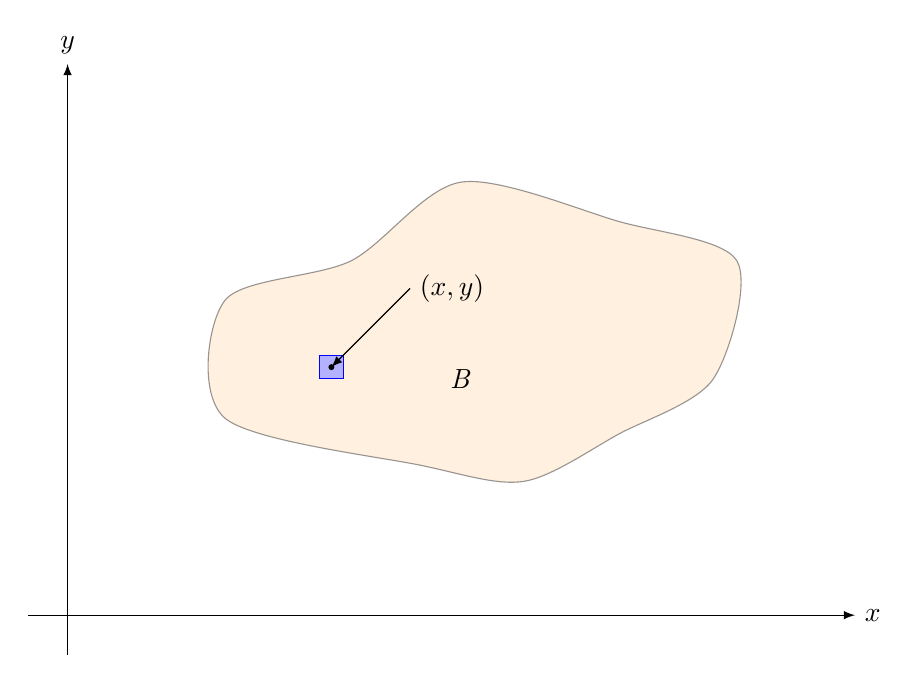
\begin{tikzpicture}
        \draw[-latex] (-0.5, 0) -- (10, 0) node[right] {$x$};
        \draw[-latex] (0, -0.5) -- (0, 7) node[above] {$y$};
        \draw[fill = orange!30, opacity = 0.4] plot [smooth cycle] 
        coordinates {(2, 2.5) (4.5, 1.9) (5.8, 1.7) (7, 2.3) (8.2, 3) 
        (8.5, 4.5) (7, 5) (5, 5.5) (3.6, 4.5) (2, 4)};
        \node[] at (5, 3) {\textit{B}};
        \draw[blue, fill = blue!30] (3.2, 3) rectangle (3.5, 3.3);
        \draw[fill = black] (3.35, 3.15) circle (0.03);
        \draw[latex-] (3.35, 3.15) -- (4.35, 4.15)  node[right] {$(x, y)$};
        
    \end{tikzpicture}
    \caption{A generic lamina that occupies the region \textit{B}}
    \label{fig:lamina}
\end{figure}

We can find the mass of the entire lamina by dividing it into many of these 
small rectangles and adding the masses of all the rectangles (see 
\ref{fig:laminagrid}). Just like in previous examples, there is some point 
$(x_{ij}^*, y_{ij}^*)$ in each rectangle, $R_{ij}$, such that the mass of the 
part of the lamina that occupies $R_{ij}$ is $\rho (x_{ij}^*, y_{ij}^*) \Delta 
A$. Adding all these masses yields:
$$m_{total} \approx \sum_{i = 1}^m \sum_{j = 1}^n \rho (x_{ij}^*, y_{ij}^*) 
\Delta A$$

Taking the limit as $m, n \to \infty$ increases the number of rectangles to 
yield the true total mass:
$$m_{total} = \lim_{m, n \to \infty} \sum_{i = 1}^m \sum_{j = 1}^n \rho (x_{ij
}^*, y_{ij}^*) \Delta A = \iint_{\textit{B}} \rho (x, y)\,dA$$

\begin{figure}[htbp]
\centering
    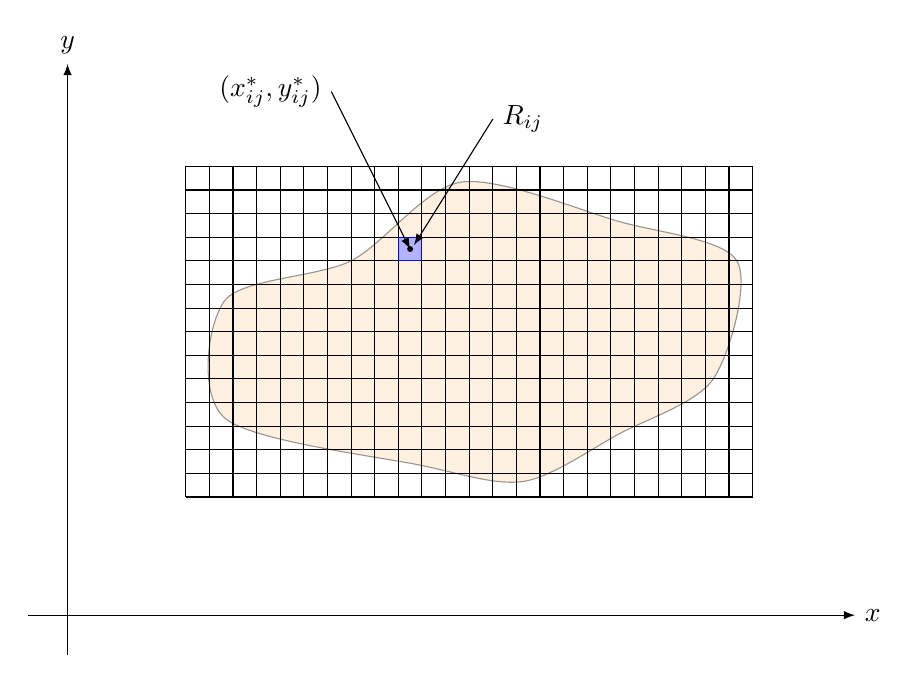
\begin{tikzpicture}
        \draw[-latex] (-0.5, 0) -- (10, 0) node[right] {$x$};
        \draw[-latex] (0, -0.5) -- (0, 7) node[above] {$y$};
        \draw[fill = orange!30, opacity = 0.4] plot [smooth cycle] 
        coordinates {(2, 2.5) (4.5, 1.9) (5.8, 1.7) (7, 2.3) (8.2, 3) 
        (8.5, 4.5) (7, 5) (5, 5.5) (3.6, 4.5) (2, 4)};
        \draw[step = 0.3] (1.5, 1.5) grid (8.7, 5.7);
        \draw[blue, fill = blue!30] (4.2, 4.5) rectangle (4.5, 4.8);
        \draw[fill = black] (4.35, 4.65) circle (0.03);
        \draw[latex-] (4.35, 4.65) -- (3.35, 6.65)  node[left] {$(x_{ij}^*, 
        y_{ij}^*)$};
        \draw[latex-] (4.4, 4.7) -- (5.4, 6.3) node[right] {$R_{ij}$};
        
    \end{tikzpicture}
    \caption{A generic lamina divided into many rectangles}
    \label{fig:laminagrid}
\end{figure}

\textbf{Example}: Find the total mass of a lamina that occupies the region 
$\textit{D} = \{ \left( x, y \right) \text{ }| \text{ } 1 \leq x \leq 3, 1 
\leq y \leq 4 \}$ with a density function $\rho (x, y) = 3y^2$. 

\textbf{Solution}: We know that the total mass is given by:
$$\iint_{\textit{D}} 3y^2\,dA$$

Applying Fubini's theorem, we see that:
$$\iint_{\textit{D}} 3y^2\,dA = \int_1^3 \int_1^4 3y^2\,dy\,dx$$
$$= \int_1^3 \left[ y^3 \right]_{y = 1}^{y = 4}\,dx = \int_1^3 \left[4^3 - 
1^3 \right]\,dx$$
$$= \int_1^3 63 \,dx = 63x|_{x = 1}^{x = 3} = 126$$

\begin{Exercise}[title = {Finding Total Mass}, label = total_mass]
Find the mass of the lamina that occupies the region, \textit{D}, and has the 
given density function, $\rho$. 
\begin{enumerate}
\item $\textit{D} = \{(x, y)\text{ }|\text{ } 0 \leq x \leq 4, 0 \leq y \leq 3 
\}; \rho (x, y) = 1 + x^2 + y^2$
\item \textit{D} is the triangular region with vertices $(0, 0)$, $(2, 1)$, 
$(0, 3)$; $\rho (x, y) = x + y$
\end{enumerate}
\end{Exercise}

\begin{Answer}[ref = total_mass]
\begin{enumerate}
    \item $\iint_{\textit{D}} \left(1 + x^2 + y^2 \right)\,dA = \int_0^4 
    \int_0^3 \left( 1  + x^2 + y^2 \right)\,dy\,dx$ $= \int_0^4 \left[y + x^2y 
    + \frac{1}{3}y^3 \right]_{y = 0}^{y = 3}\,dx$ $= \int_0^4 \left[ 3 + 3x^2 
    + \frac{1}{3}(3)^3 \right]\,dx$ $= \int_0^4 \left(12 + 3x^2 \right)\,dx$ 
    $= \left[ 12x + x^3 \right]_{x = 0}^{x = 4} = 12(4) + 4^3 = 112$
    \item First, let's visualize this region, since it isn't a rectangle:
    
    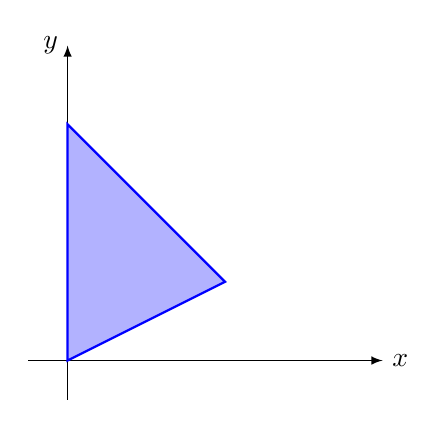
\begin{tikzpicture}
        \centering
        \draw[-latex] (-0.5, 0) -- (4, 0) node[right] {$x$};
        \draw[-latex] (0, -0.5) -- (0, 4) node[left] {$y$};
        \draw[thick, blue, fill = blue!30] (0,0) -- (2, 1) -- (0, 3) -- cycle;
    \end{tikzpicture}

    Let's divide the triangle horizontally and write equations for each of the 
    sides that do not lie on the $y$-axis.

    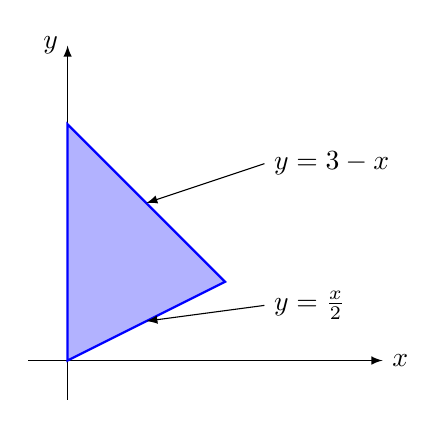
\begin{tikzpicture}
        \centering
        \draw[-latex] (-0.5, 0) -- (4, 0) node[right] {$x$};
        \draw[-latex] (0, -0.5) -- (0, 4) node[left] {$y$};
        \draw[thick, blue, fill = blue!30] (0,0) -- (2, 1) -- (0, 3) -- cycle;
        \draw[latex-] (1, 0.5) -- (2.5, 0.7) node[right] {$y = \frac{x}{2}$};
        \draw[latex-] (1, 2) -- (2.5, 2.5) node[right] {$y = 3 - x$};
    \end{tikzpicture}

    We see that we can describe region \textit{D} as $\textit{D} = \{ (x, y) 
    \text{ }|\text{ } 0 \leq x \leq 2, \frac{x}{2} \leq y \leq 3 - x\}$. 
    Therefore $\iint_{\textit{D}} \left( x + y \right) \,dA$ $= \int_0^3 \int_{
    x/2}^{3 - x} \left(x + y \right)\,dy\,dx$ $= \int_0^3 \left[xy + 
    \frac{1}{2} y^2 \right]_{y = x/2}^{y = 3 - x}\,dx$ $= \int_0^3 \left[ 
    \left(x(3 - x) \right) - \left(x (x/2) \right) + \frac{1}{2} \left( (3 - 
    x)^2 - (x/2)^2 \right) \right]\,dx$ $= \int_0^3 \left[ \left(3x - x^2 - 
    \frac{x^2}{2} \right) + \frac{1}{2} \left( 9 - 6x + x^2 - \frac{x^2}{4} 
    \right) \right]\,dx$ $= \int_0^3 \left[-x^2 - \frac{x^2}{2} + \frac{x^2}{2}
    - \frac{x^2}{8} + 3x - 3x + \frac{9}{2} \right]\,dx$ $= \int_0^3 \left( -
    \frac{9x^2}{8} + \frac{9}{2} \right)\,dx$ $= \left[ \frac{9x}{2} -\frac{
    3x^3}{8} \right]_{x = 0}^{x = 2}$ $= \frac{9(2)}{2} - \frac{3(8)}{8} = 9 - 
    3 = 6$
\end{enumerate}
\end{Answer}

This method applies not only to mass density, but any other type of density. 
Some examples could include animals per acre of forest, cells per square 
centimeter of petri dish, or people per city block. A density physicists are 
often interested in is charge density (that is, the amount of charge, $Q$, per 
unit area). Charge is measured in coulombs (C). Often, charge density is given 
by a function, $\sigma (x, y)$, in units of coulombs per area (such as 
$\text{cm}^2$ or $\text{m}^2$). If there is some region, \textit{D}, with 
charge distributed across it such that the charge density can be described 
by a continuous function, $\sigma (x, y)$, then the total charge, Q, is given 
by:
$$Q = \iint_{\textit{D}} \sigma (x, y)\,dA$$

\textbf{Example}: Charge is distributed over the region \textit{B} shown in 
figure \ref{fig:charge} such that the charge density is given by $\sigma (x, y)
= xy$, measured in C/$\text{m}^2$. Find the total charge. 

\begin{figure}[htbp]
\centering
    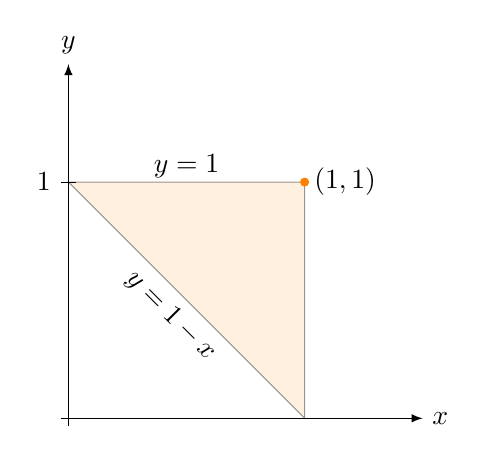
\begin{tikzpicture}
        \draw[-latex] (-0.1, 0) -- (4.5, 0) node[right] {$x$};
        \draw[-latex] (0, -0.1) -- (0, 4.5) node[above] {$y$};
        \draw[fill = orange!30, opacity = 0.4] (3, 0) -- (3, 3) -- (0, 3) -- 
        cycle;
        \draw[orange, fill = orange] (3, 3) circle (0.05) node[black, right] 
        {$(1, 1)$};
        \draw[] (0.1, 3) -- (-0.1, 3) node[left] {$1$};
        \node[] at (1.5, 3.2) {$y = 1$};
        \node[rotate = -45] at (1.3, 1.3) {$y = 1 - x$};
        
    \end{tikzpicture}
    \caption{A triangular region over which charge is distributed such that 
    $\sigma (x, y) = xy$}
    \label{fig:charge}
\end{figure}

\textbf{Solution}: We know that total charge is given by:
$$Q = \iint_{\textit{B}} xy\,dA$$ 

Examining figure \ref{fig:charge}, we see that:
$$\iint_{\textit{B}} xy\,dA = \int_0^1 \int_{1 - x}^1 xy\,dy\,dx$$
$$= \int_0^1 \frac{x}{2} \left[ y^2 \right]_{y = 1 - x}^{y = 1}\,dx = \int_0^1 
\frac{x}{2} \left[ 1^2 - \left( 1 - x \right)^2 \right]\,dx$$
$$= \frac{1}{2} \int_0^1 x \left(1 - 1 + 2x - x^2 \right)\,dx = \frac{1}{2} 
\int_0^1 x \left(2x - x^2 \right)\,dx$$
$$= \frac{1}{2} \int_0^1 2x^2 - x^3\,dx = \frac{1}{2} \left[ \frac{2}{3}x^3 - 
\frac{1}{4}x^4 \right]_{x = 0}^{x = 1} = \frac{1}{2} \left( \frac{2}{3} - 
\frac{1}{4} \right) = \frac{5}{24} \text{C}$$


\subsection{Center of Mass}

\subsection{Moment of Inertia}

\subsection{Surface Area}

\section{Triple Integrals}
